\subsection{Introduction}
	This section is divided in two parts, the first one describe the implementation of the algorithm in a laptop computer. The objective is to get a reference to compare the results of the final implementation. The second one is a description of the final application and its results.
	During this experiments, five datasets were used. These datasets were provided by the GRVC, captured in the testbed of CATEC \cite{CATEC}, and were used previously by a partner. These datasets, composed by a number of images and data provided by a VICON system (Time, position and orientation of quadrotors), and Representing different situations, yielded a number of interesting results that will be gathered at the end of this chapter. 

	\begin{figure}[h]
		\centering
		\begin{subfigure}{0.49\linewidth}
			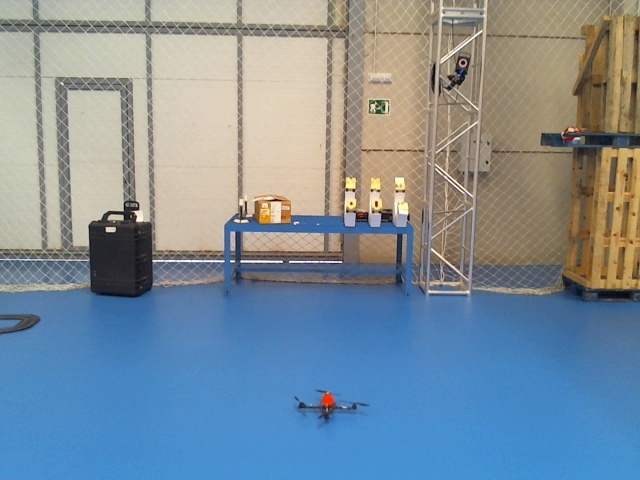
\includegraphics[width=\linewidth]{../Images/c4/image_ori}
			\caption{Original Image}
			\label{fig:image_ori}
		\end{subfigure}
		%--------------------------------------------------------------------
		\begin{subfigure}{0.49\linewidth}
			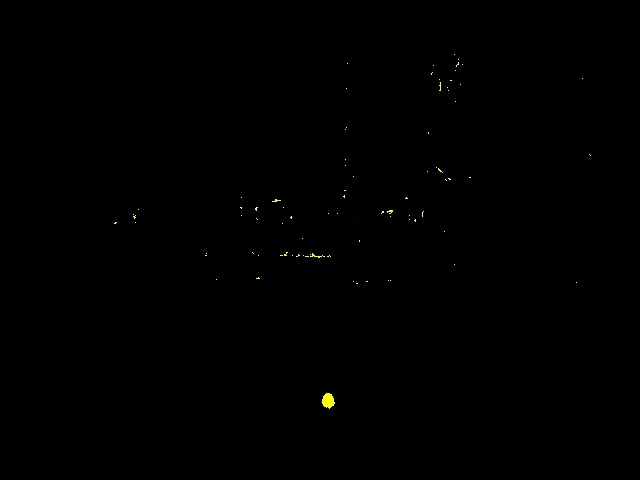
\includegraphics[width=\linewidth]{../Images/c4/image_seg}
			\caption{Segmented Image}
			\label{fig:image_seg}
		\end{subfigure}
		\caption{Images to and from algorithm}
		\label{fig:frames_PC}
	\end{figure}

	Figure: \ref{fig:frames_PC} shows an example of captured image from the camera and the result of the segmentation algorithm. Particularly, we were looking for orange color (The cap of the quadrotor in this case). However unlike simulation, where there was only one object as the result of segmentation, the algorithm return many targets. The first sift is by size, we do not consider tiny objects that use to be noise and are quantitative smaller than the target.
		
	
	Following sections shows the results of the described algorithm while running completely on the same computer and afterwards using the definitely structure of the system (Ground Station on PC and the capture and segmentation on the on-board computer) with the provided datasets.

\subsection{Complete Test in PC}
	PC's and other's characteristics:
	\begin{itemize}
		\item{Pictures of 640x480}
		\item{Intel core i7 2.20 GHz. Usage 7-10\%}
		\item{6 GB of RAM. Usage $\sim$ 5000-7000 KB}
	\end{itemize}
	\subsubsection{Ground Tracking algorithm}
	
	All datasets have information about two cameras tracking a target. However, in this experiment, we use only the information about the first  of the camera. The following table shows the medium time and speed of every step of the algorithm: \\
	
	{
	\centering
		\begin{tabular}{|c|c|c|c|c||c|}
		\hline  					&  Open Image	&  RGB to HSV 	& Segmentation 	& EKF step  & Complete \\ 
		\hline  \textbf{time (ms)}	& 0.0085 		& 0.0015 		& 0.0100 		& 0.0001 	& 0.0231 	\\ 
		\hline  \textbf{fps (1/s)}	&  118			&  645			&  100			& 13936 	& 43 		\\ 
		\hline 
		\end{tabular} 
	}
	\newline

	{
	\label{Reference_fps_table}
	This application runs sequentially, so the "complete"\footnote{The complete time has a higher value, than the addition of the previous, because it includes some GUI process} time of the process is the addition of the previous ones. Therefore, It is possible to reduce the complete process time using multi-threading (or in other words increase the FPS). In the following section will be described the results of the process with multi-threading inside the on-board computer. \ref{test_with_odroid_and_GT}
	}
	
	The next graphs shows the original and estimated position of the target \ref{fig:trajectories_PC} and the error between both \ref{fig:errors_PC}. In general terms, the errors associated with each axis are bounded below 0.2 m.
	
	\begin{figure}[hp]
		\centering
		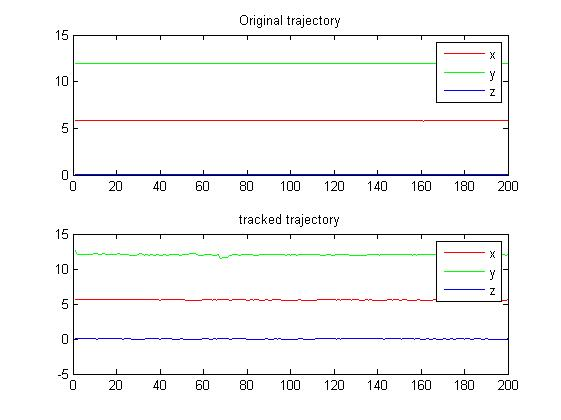
\includegraphics[width=0.75\linewidth]{../Images/c4/trajs}
		\caption{Original and tracked trajectories}
		\label{fig:trajectories_PC}
	\end{figure}
	
	\begin{figure}[hp]
		\centering
		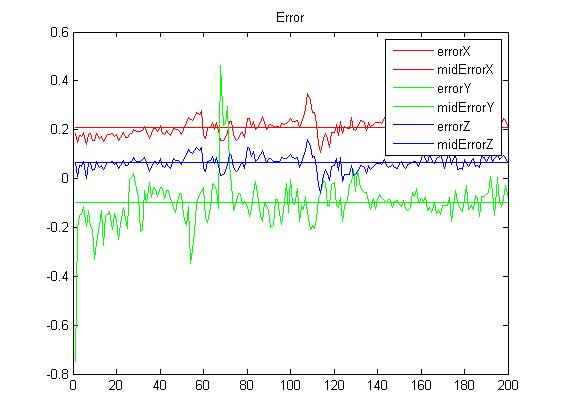
\includegraphics[width=0.5\linewidth]{../Images/c4/errors}
		\caption{Error between real and tracked trajectories}
		\label{fig:errors_PC}
	\end{figure}
	
	\newpage
	
	%\begin{figure}[ht]
	%	\centering
	%	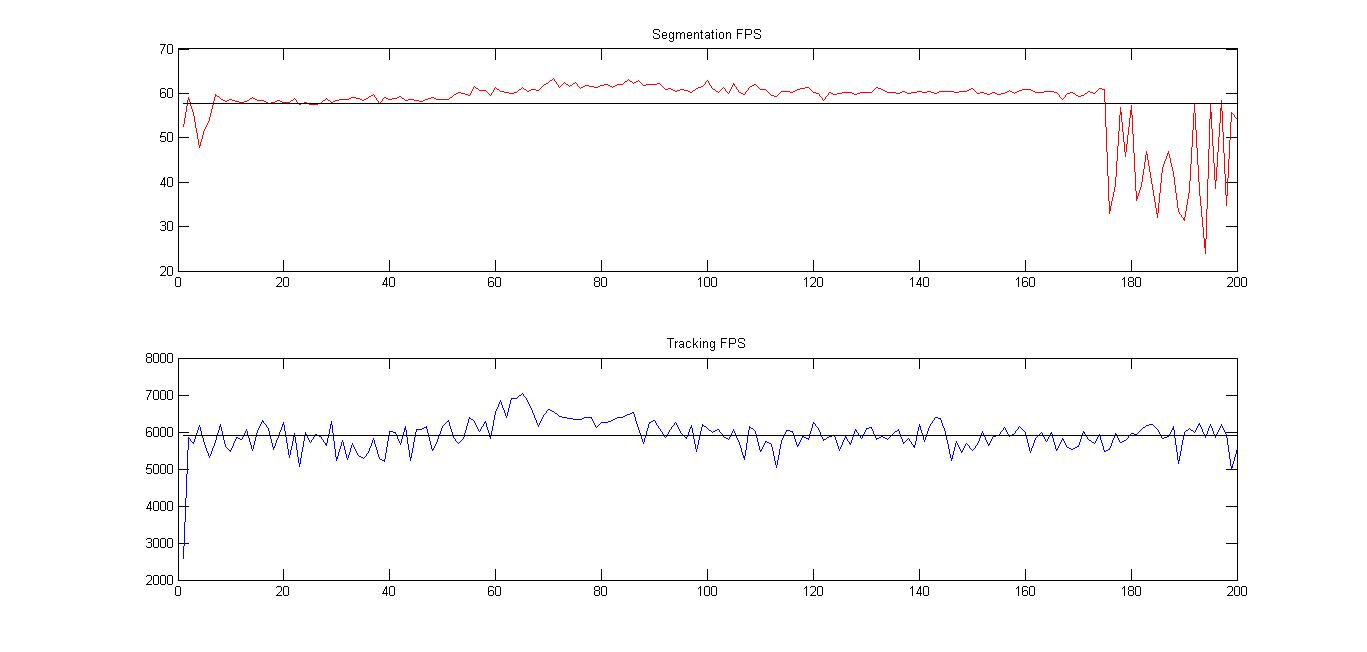
\includegraphics[width=\linewidth]{../Images/c4/fps}
	%	\caption{}
	%	\label{fig:fps_PC}
	%\end{figure}
		
	\subsubsection{Stereo Tracking algorithm}
	
	On this case, we use the data about both of the cameras. As previously, the following table collect time information about the process of the application. \\
		
	{                
	\centering
		\begin{tabular}{|c|c|c|c|c||c|}
		\hline  					&  Open Image	&  RGB to HSV 	& Segmentation 	& EKF step  & Complete \\ 
		\hline  \textbf{time (ms)}	&	0.0222		& 	0.0031 		&  	0.0157		&  	0.0001 	&  0.0429		\\ 
		\hline  \textbf{fps (1/s)}	& 	45 			& 	321.5 		& 	63.8 		& 9785.5	&  23.3		\\ 
		\hline 
		\end{tabular} 
	}
	\newline
	
	This table has the same annotation that the previous one \ref{Reference_fps_table}.
	
	Eventually, these figures shows the position of the target, the result of the estimation \ref{fig:trajectories_stereo_PC} and the error between both \ref{fig:errors_stereo_PC}.
	
	\begin{figure}[hp]
		\centering
		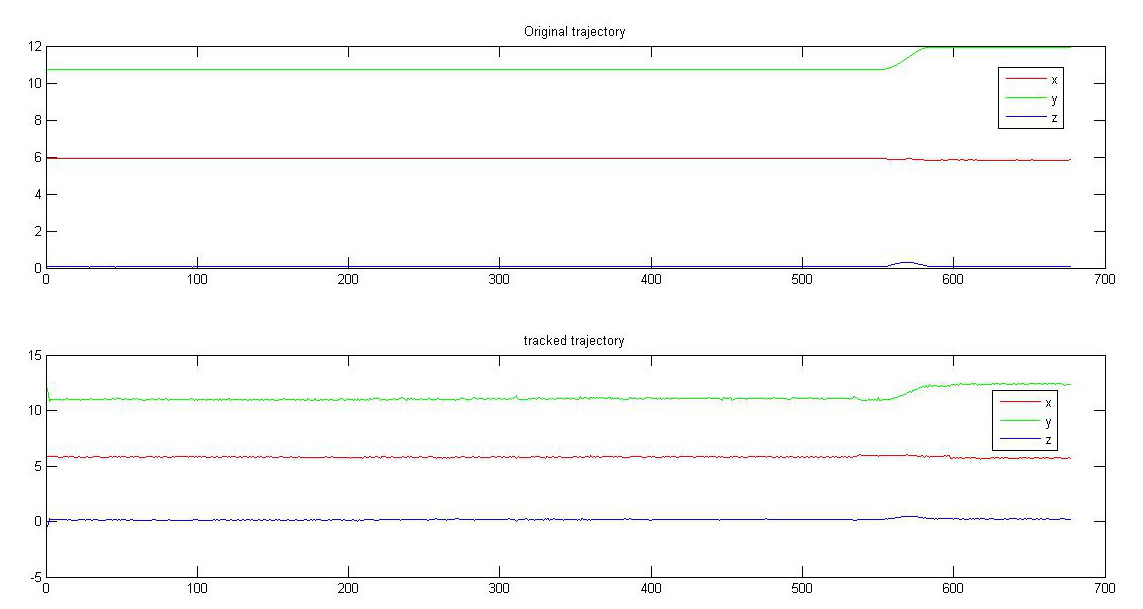
\includegraphics[width=\linewidth]{../Images/c4/trajs_stereo}
		\caption{Original and tracked trajectories}
		\label{fig:trajectories_stereo_PC}
	\end{figure}
	
	\begin{figure}[htp]
		\centering
		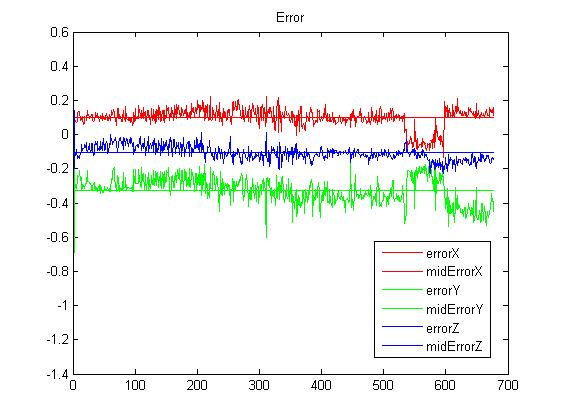
\includegraphics[width=0.7\linewidth]{../Images/c4/errors_stereo}
		\caption{Error between real and tracked trajectories}
		\label{fig:errors_stereo_PC}
	\end{figure}	
	
	\newpage
	
\subsection{Test with Odroid and Ground Station}
	\label{test_with_odroid_and_GT}
	
	\begin{wrapfigure}{r}{0.5\linewidth}
		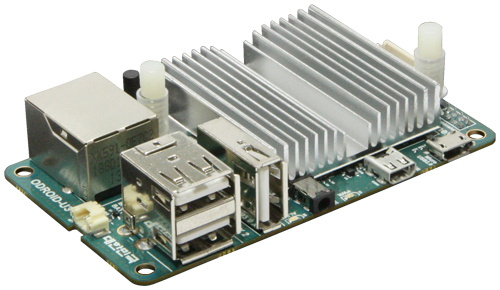
\includegraphics[width=\linewidth]{../Images/c4/odroidu3}
		\caption{Hardkernel Odroid u3}
		\label{fig:odroidu3}
	\end{wrapfigure}
		
	The result of this sections where obtained from two application. The first is the Ground Station application, which were running in the same computer of the previous section. This PC was connected to a local network (Router). The architecture of this app.  was described in figure \ref{fig:GroundStation}
	
	The second application were running inside the on-board computer \ref{fig:Quadsoftware} connected by WiFi to the same network. Particularly, the on-board computer is a Hardkernel Odroid-u3 with the following characteristics:
	
	
	\begin{itemize}
		\item 1.7GHz Quad-Core processor 
		\item 2GB RAM
		\item GPU ARM Mali-400 Quad Core 440MHz  
	\end{itemize}
	
	As described in section \ref{sec:SoftArch}, the quad handles the capture and treatment of pictures and eventually send the information to the Ground Station. After that, the Ground Station process the data and store the information. The only difference is that, instead of capturing the photos, the quad open the images from the data set.
	
	
	\subsubsection{Ground Tracking algorithm}
	
	The first test case was (As in previous sections), the tracking of a single ground target. The following table got the timing information of the process. It's important to mention that the application has the four different threads mentioned previously \ref{itemize:quadappthreads}. That means that unlike the previous section, the execution time is not sequential but parallel. So the complete process time is not the summarize of each process's time.
	
	Attending to the quadrotor's application, the following table gather some process's duration and it speed:
	% 666 TODO: quitar el filtro de media del tratamiento que ralentiza mucho
	\newline
	\newline
	{
	\centering
		\begin{tabular}{|c|c|c|c|c|c|}
		\hline  					&  Open Img	&  cp Img 	& Vicon 	& Treat img & Comm  		\\ 
		\hline  \textbf{time (ms)}	& 	0.0154	& 0.0018	&	0.00096	&  	 0.019	&	0.0001		\\ 
		\hline  \textbf{fps (1/s)}	&  	68		&  63.2		&  10356	&  	51.23	&	12022		\\ 
		\hline 
		\end{tabular} 
	}
	\newline
	
	This second table gather the time information in the Ground Station application:
	\newline
	
	{
	\centering
		\begin{tabular}{|c|c|c|}
		\hline  					&  comm		&  EKF step	\\
		\hline  \textbf{time (ms)}	& 	0.0001	& 	0.0001	\\
		\hline  \textbf{fps (1/s)}	&  	10567.5	&  	9608.5	\\
		\hline 
		\end{tabular} 
	}
	\newline
	
	The higher computational cost is the image capture and segmentation, by the quadcopter. Due to the lower computational characteristics of the on-board pc the speed of the algorithm is slightly reduced.
	
	Finally, the following figure \ref{fig:arch_trajs} shows the original trajectory and the tracked one. Should be noted that the amount of info used by the tracker is lower than the provider by the dataset. That's because the asynchronism, if some new info if get before been processed the application process the last one in order to work with the newest data as possible. The medium error is $\sim$ 0.2m as in the previous tests.
	
	\begin{figure}[ph]
		\centering
		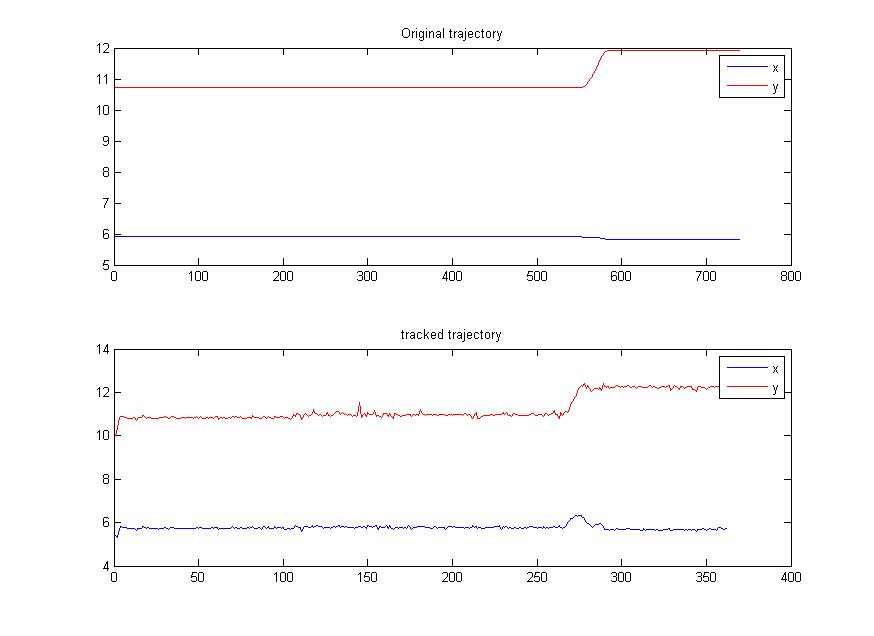
\includegraphics[width=0.7\linewidth]{../Images/c4/arch_trajs}
		\caption{Original and tracked trajectories}
		\label{fig:arch_trajs}
	\end{figure}

	
	\subsubsection{Stereo Tracking algorithm}
		Attending to the quadrotor's application, the following table gather some process's duration and it speed:
		% 666 TODO: quitar el filtro de media del tratamiento que ralentiza mucho
		\newline
		\newline
		{
		\centering
			\begin{tabular}{|c|c|c|c|c|c|}
			\hline  					&  Open Img	&  cp Img 	& Vicon 	& Treat img & Comm  		\\ 
			\hline  \textbf{time (ms)}	& 	0.0161	& 0.0019	&	0.000098&  	 0.02	&	0.0001		\\ 
			\hline  \textbf{fps (1/s)}	&  	62.11	&  52.631	& 10204.08 	&  49.56	&	986.1	\\ 
			\hline 
			\end{tabular} 
		}
		\newline
		
		This second table gather the time information in the Ground Station application:
		\newline
		
		{
		\centering
			\begin{tabular}{|c|c|c|}
			\hline  					&  comm		&  EKF step	\\
			\hline  \textbf{time (ms)}	& 	0.0001	& 	0.0001	\\
			\hline  \textbf{fps (1/s)}	&  	10368.5	&   9898.6 	\\
			\hline 
			\end{tabular} 
		}
		\newline
	\begin{figure}[ph]
		\centering
		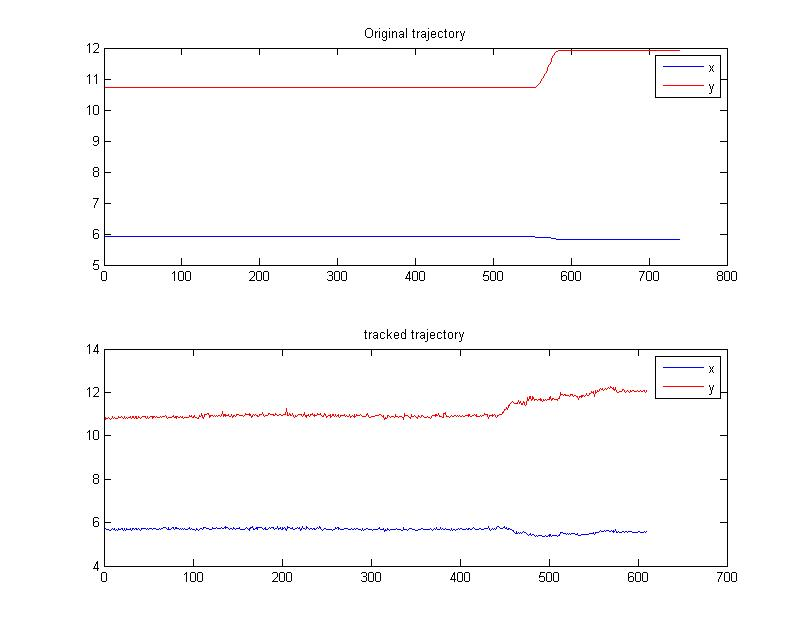
\includegraphics[width=0.7\linewidth]{../Images/c4/arch_trajs_stero}
		\caption{Original and tracked trajectories}
		\label{fig:arch_trajs_stero}
	\end{figure}
	
	\begin{figure}[ph]
		\centering
		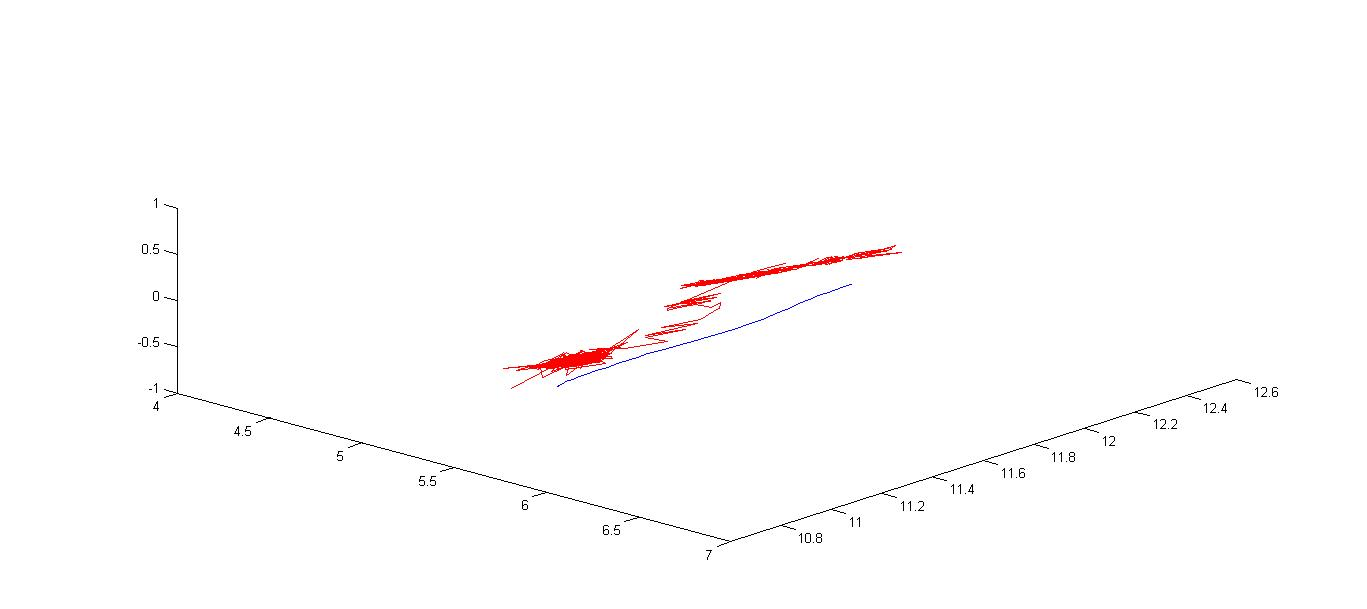
\includegraphics[width=0.6\linewidth]{../Images/c4/arch_3d_trajs_stero}
		\caption{3d trajectories}
		\label{fig:arch_3d_trajs_stero}
	\end{figure}
